\chapter{Resultados}

Analisando primeiro os resultados obtidos com os parâmetros originais 
do artigo de Parham e Michael ($T_1=23.2, \ T_2=0.07, \ \omega_1=0.67, 
\ \phi_1=1.53, \ R_1=85.9, \ R_2=0.98, \ \omega_2=0.65, \ \phi_2=1.99, 
\ A=-0.03, \ B=1.31, \ C=-4.4, \ b_1=0.04, \ b_2 = 0.09, \ T_{min}=14.5, 
\ \gamma= 1/120,\ R_L = 50, \ c_1=0.00554, \ c_2=-0.06737$ \cite{Parham2010}, \cite{OKUNEYE201772}), 
e utilizando a população média estimada anteriormente e um valor arbitrário 
para a população de mosquitos, de 10000, assumindo 1000 humanos infectados 
e 5000 mosquitos expostos à malária em $t=0$, a modelagem ficou como a seguir 
\footnote{A elaboração do modelo com os dados originais pode ser encontrada em
https://github.com/RaphaLevy/TCC/blob/main/old/Dados\%20Originais.ipynb.}: 

% Pra plotar duas imagens uma ao lado da outra, precisa corrigir a posição das legendas.

% \begin{figure}
% \hspace*{-1.5cm} % Adiciona espaço negativo para puxar a imagem para a esquerda
% \begin{minipage}{.45\textwidth}
%   \centering
%   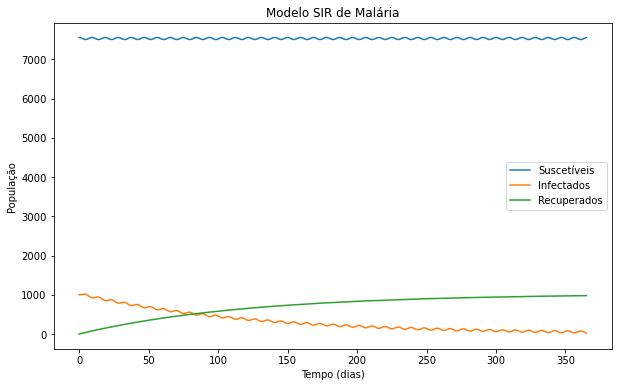
\includegraphics[width=1.25\linewidth]{SIR_Dados_Originais_Parham_Michael.png}
%   \captionof{figure}{A figure}
%   \label{fig:test1}
% \end{minipage}%
% \hspace{1.5cm} % Adiciona espaço horizontal
% \begin{minipage}{.45\textwidth}
%   \centering
%   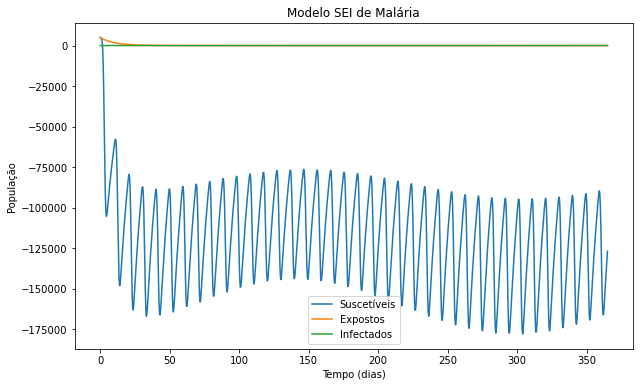
\includegraphics[width=1.3\linewidth]{SEI_Dados_Originais_Parham_Michael.png}
%   \captionof{figure}{Another figure} % Legenda à direita da segunda imagem
%   \label{fig:test2}
% \end{minipage}
% \end{figure}





\begin{figure}[!ht]
        \centering
        \hbox{\hspace{4em} 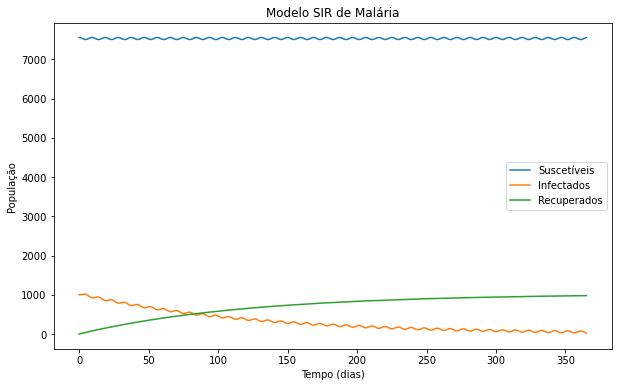
\includegraphics[scale=0.5] {SIR_Dados_Originais_Parham_Michael.png}}
        \caption{SIR com dados originais}
\end{figure} 
\begin{figure}[!ht]
        \centering
        \hbox{\hspace{3em} 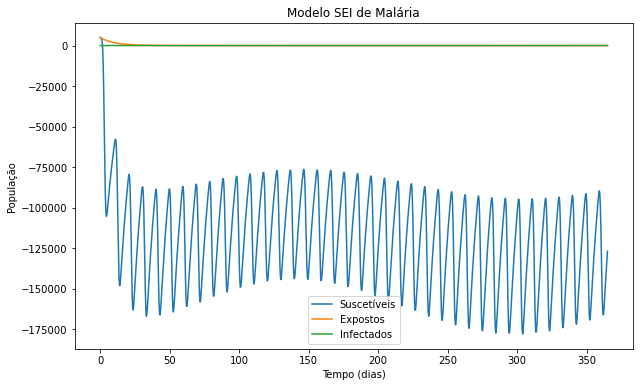
\includegraphics[scale=0.5] {SEI_Dados_Originais_Parham_Michael.png}}
        \caption{SEI com dados originais}
\end{figure} 
\newpage
Com essa modelagem inicial, é perceptível uma forte oscilação do número de humanos e mosquitos suscetíveis, assim como de humanos infectados. Ademais, é notável que, com esses parâmetros, a epidemia não irá se estabilizar, visto que o número de humanos infectados tende a 0 ao longo do ano, enquanto que a população de mosquitos suscetíveis fica negativa e a população de expostos e infectados também tende a 0. Esses efeitos foram caracterizados pela temperatura e precipitação oscilando em períodos de tempo muito curtos, devido a um alto valor de $\omega$ para ambas as funções. 
\\\\
Coletando dados climatológicos de Manaus em \cite{ClimaMANAUS}, a temperatura e precipitação média foram estimados como 26.4 $^\circ C$ e 250.083 mm, respectivamente. Com esses dados, a amplitude da variabilidade sazonal, frequência angular e ``phase lag" da variabilidade para ambos foram definidos de forma a aproximar os valores reais:
\\\\
\begin{adjustwidth}{-0.5cm}{}
\begin{center}
\renewcommand{\arraystretch}{1.5}
\begin{tabular}{|c | c|} 
 \hline
 \textbf{Parâmetro} & \textbf{Valor}\\ 
 \hline
  $T_1$ & \makecell[l]{\rule{0pt}{3ex}26.4$^\circ C$\rule[-1.5ex]{0pt}{0pt}} \\
 \hline
 $T_2$ & \makecell[l]{\rule{0pt}{3ex}0.025\rule[-1.5ex]{0pt}{0pt}} \\
 \hline
 $\omega_1$ & \makecell[l]{\rule{0pt}{3ex}0.017 (meses)$^{-1}$\rule[-1.5ex]{0pt}{0pt}} \\
 \hline
 $\phi_1$ & \makecell[l]{\rule{0pt}{3ex}-1.45\rule[-1.5ex]{0pt}{0pt}} \\
 \hline
 $R_1$ & \makecell[l]{\rule{0pt}{3ex}250.083 mm\rule[-1.5ex]{0pt}{0pt}} \\
 \hline
 $R_2$ & \makecell[l]{\rule{0pt}{3ex}0.565\rule[-1.5ex]{0pt}{0pt}} \\
 \hline
 $\omega_2$ & \makecell[l]{\rule{0pt}{3ex}0.02 (meses)$^{-1}$\rule[-1.5ex]{0pt}{0pt}} \\
 \hline
 $\phi_2$ & \makecell[l]{\rule{0pt}{3ex}1.6\rule[-1.5ex]{0pt}{0pt}} \\
 \hline
\end{tabular}
\captionof{table}{Valores dos parâmetros de clima}
\end{center}
\end{adjustwidth}

\vspace{1cm}
Os parâmetros de amplitude ($T_2$ e $R_2$) e defasagem de fase 
($\phi_1$ e $\phi_2$) são adimensionais. A temperatura e precipitação ao 
longo do ano evoluem então da seguinte maneira\footnote{A elaboração dos gráficos pode ser encontrada em
\\
https://github.com/RaphaLevy/TCC/blob/main/Discuss\%C3\%A3o/Correcao\_de\_Modelagens.ipynb}:


% \begin{figure}
% \hspace*{-1.5cm} % Adiciona espaço negativo para puxar a imagem para a esquerda
% \begin{minipage}{.45\textwidth}
%   \centering
%   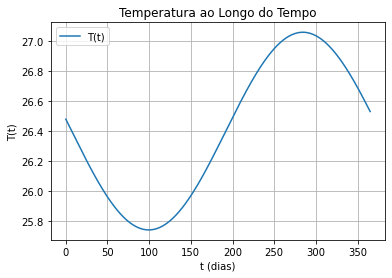
\includegraphics[width=1.2\linewidth]{Grafico_da_Temperatura.png}
%   \captionof{figure}{A figure}
%   \label{fig:test1}
% \end{minipage}%
% \hspace{1.5cm} % Adiciona espaço horizontal
% \begin{minipage}{.45\textwidth}
%   \centering
%   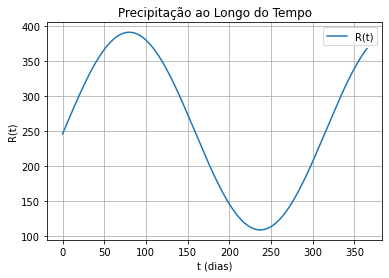
\includegraphics[width=1.2\linewidth]{Grafico_da_Precipitacao.png}
%   \captionof{figure}{Another figure} % Legenda à direita da segunda imagem
%   \label{fig:test2}
% \end{minipage}
% \end{figure}


\begin{figure}[!ht]
        \centering
        \hbox{\hspace{7.2em} 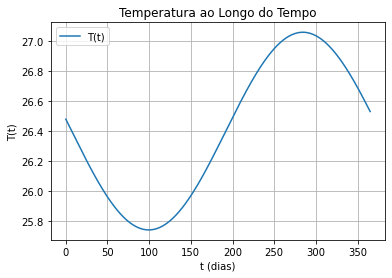
\includegraphics[scale=0.6] {Grafico_da_Temperatura.png}}
        \caption{Gráfico da temperatura}
\end{figure} 
\newpage
\begin{figure}[!ht]
        \centering
        \hbox{\hspace{7.5em} 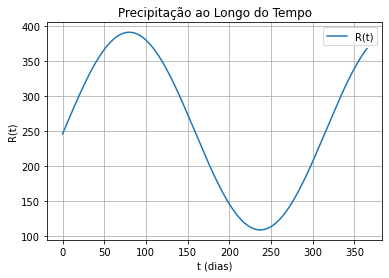
\includegraphics[scale=0.6] {Grafico_da_Precipitacao.png}}
        \caption{Gráfico da precipitação}
\end{figure} 
De forma a garantir a corretude da função com os parâmetros utilizados, calculei os valores da temperatura nos meses de outubro e maio, 
que são o mais quente e frio do ano, com temperaturas médias de 27.6 $^\circ C$ e 25.8 $^\circ C$ respectivamente, e da precipitação em 
março e agosto, que são os meses com maior e menor precipitação, com 395 e 114 mm, respectivamente. Os valores médios obtidos foram de 
27.06 $^\circ C$, 25.86 $^\circ C$, 390.67 mm e 112.89 mm. Tendo os parâmetros de $T$ e $R$ prontos para uma primeira análise, a evolução 
das populações de humanos e mosquitos foram verificadas utilizando $N=8558$, 
com $S_{H0} = 7558$, $I_{H0} = 10000$, $M= 300000$, $S_{M0}=250000$, $E_{M0} = 50000$, $A = 317.925, \ B = 15, \ C = -48.78$ e $R_L = 312 \ \text{mm}$. 
Os resultados podem ser encontrados no Apêndice 1 e 2 \footnote{A elaboração dos gráficos acima pode ser encontrada em
\\
https://github.com/RaphaLevy/TCC/blob/main/old/Testa\_Infectados\_Humanos.ipynb}. 
\\\\
Notavelmente, a modelagem resultante não está correta, com ambas as populações se tornando negativas em certos pontos, especialmente a da população humana, cujo número de infectados decai para aproximadamente -300000. Verificando as EDOs, foi possível ver que o único parâmetro que é dado em função da temperatura e chuva no SIR é o $a(T)$, que é a taxa de picadas por dia. Dada a sua fórmula, e sabendo que a temperatura inicialmente decai nos primeiros meses do ano, tem-se que $a$ tomará valores negativos na equação de infectados, visto que $T_1$ será maior que $T$ inicialmente, explicando o comportamento da curva. Se comparado com os dados do artigo de Parham e Michael, cuja temperatura é crescente inicialmente, foi necessário modificar a ordem do numerador dessa taxa para que, num primeiro momento, não se torne negativa conforme a temperatura decai. Utilizando então a equação $a(T) = \dfrac{T_1-T}{D_1}$, os resultados podem ser vistos no apêndice 3 e 4.
\\\\
Com essas modificações, a evolução da população humana parece mais viável do que estava anteriormente, com o número de infectados inicialmente baixo, 
aumentando ao longo do ano e posteriormente decaindo. Por outro lado, é possível notar que próximo do tempo final de análise, o número de humanos 
infectados se torna negativo. A modelagem de mosquitos, por sua vez, se manteve relativamente estável.
\\\\
Analisando o comportamento da modelagem de mosquitos de forma que a população ficasse aproximadamente constante ao longo do período, dadas as equações diferenciais do modelo SEI, e os parâmetros passados para atingir esse objetivo, o valor de $\mu$ passado fica muito próximo de 0, enquanto que $l(\tau_M)$, uma probabilidade, fica muito próxima de 1. Por isso, $\dfrac{dE_M}{dt}$ também fica bem próximo de 0, fazendo com que a função de expostos seja linear, aproximadamente constante no número inicial de infectados, enquanto que a população de mosquitos que sai do compartimento de suscetíveis quase que simultaneamente entra no compartimento de infectados, causando as ondulações espelhadas de $S$ e $I$. Para contornar esse efeito, foi necessário modificar o uso de $b_1$, para passar apenas mosquitos do compartimento $S$ para $E$, necessitando da inclusão de um novo parâmetro, $b_3$, para passar mosquitos do compartimento $E$ para $I$. Essa taxa é inversa ao período de incubação, então definimos
\begin{gather*}
    b_3 = \dfrac{T-T_{min}}{DD}
\end{gather*}
Ademais, foi removido o parâmetro $a(T)$ na passagem de mosquitos expostos para infectados, visto que nessa mudança do compartimento $E$ para $I$ não ocorrem novas picadas, assim como o parâmetro $T_1$ utilizado na fórmula de $a(T)$ também teve de ser modificado, visto que o artigo original aplica $T_1$ com dois valores diferentes, para a taxa de picadas e para a equação da temperatura por tempo. Com o intuito de manter a formatação de $T(t)$ e $R(t)$ a mesma, $T_1$ de $a$ foi modificado para $T'$.
\\\\
Considerando então o que foi dito acima, também se tornou necessário modificar as equações diferenciais do SEI, que ficaram dessa forma:
\begin{gather*}
\begin{cases}
\dfrac{dS_M}{dt} = b - ab_1\bigg(\dfrac{I_H}{N}\bigg)S_M - \mu S_M\\
\\
\dfrac{dE_M}{dt} = ab_1\bigg(\dfrac{I_H}{N}\bigg)S_M - \mu E_M - b_3E_Ml\\
\\
\dfrac{dI_M}{dt} = b_3E_Ml -\mu I_M\\
\end{cases}
\end{gather*}
\\\\
Com as adaptações feitas à transmissão da doença entre os mosquitos 
(Apêndices 5 e 6), é possível ver que não só o 
equilíbrio mudou, de forma que agora o número de 
expostos tende a 0, e não o de infectados, podemos ver também que a população 
de humanos é fortemente impactada, novamente oscilando constantemente, e com 
o número de infectados ficando negativo repetidas vezes \footnote{Observação: 
as modelagens do SIR mostradas ao longo de 5 anos de análise foram feitas 
usando o valor médio estimado para a população no período entre 2004 e 2008, 
com $N$=8558}.
Analisando modificações nos parâmetros empíricos citados acima, foi notado que esse comportamento se dá devido em especial ao alto valor em módulo de $A$, visto que com $A=-217.925$, o comportamento do modelo foi similar. Até mesmo usando $A=17.925$, o comportamento observado foi similar. Contudo, para $A=0$, a população humana teve um comportamento bem mais viável, enquanto que a população de mosquitos tendeu à extinção (Apêndices 7 e 8).
\footnote{A elaboração dos gráficos indicados acima pode ser encontrada em
\\
https://github.com/RaphaLevy/TCC/blob/main/Discuss\%C3\%A3o/Correcao\_de\_Modelagens\_2.ipynb}
\\\\
Analisando o efeito de $A$, notou-se que, para $A$ muito grande, $\mu$ se torna extremamente pequeno:
\begin{flalign*}
& \text{Para A} = 317.925, \ \mu = 4.505961269611858e-06 \\
& \text{Para A} = 17.925, \ \mu = 7.78802370175753e-05 \\
& \text{Para A} = -217.925, \ \mu = -6.599014101979344e-06 \\
& \text{Para A} = 0, \mu = 0.0028800184321179124
\end{flalign*}
Com isso, a mortalidade de mosquitos será extremamente baixa para valores 
grandes de $A$, positivos ou não. Contudo, como uma forma de possibilitar 
o uso de valores altos para esse parâmetro, e ainda garantir que as 
populações tenham valores sempre não-negativos, foi aplicado um máximo 
nas taxas com subtração, segundo recomendação do orientador, de forma que 
o valor resultante entre $T(t)-T_{min}$, $R_L - R(t)$ e $T'-T(t)$ seja o máximo entre essas diferenças e uma tolerância pequena, no caso 
foi utilizado um $\epsilon = 10^{-5}$. Isso foi suficiente para garantir que, 
mesmo com valores grandes de $A$, o modelo não tomasse valores 
negativos (Apêndices 9 a 12). 
\\\\
Com essas modificações, é possível notar como, independente do valor de $A$, a evolução das populações humanas será bem similar, com uma estabilização da população de suscetíveis logo antes de se tornar 0. A de mosquitos, por sua vez, é menos oscilante para valores grandes de $A$, e não se estabiliza mesmo em mais de 10000 dias. Por outro lado, se $A=0$, a população de mosquitos se aproxima da extinção, com pequenos picos de mosquitos unicamente suscetíveis, sem estabilização da doença. Contudo, ainda que usando o máximo entre um pequeno $\epsilon$ e as diferenças notadas acima, $T'=26.4$ é um valor menor que a temperatura máxima calculada para o ano, que é próxima de 27.1. Assim, foi recomendado pelo orientador que fosse testado um valor maior que esse máximo, no caso $T'=27.4$ (Apêndice 13 e 14).
\\\\
Tendo então o modelo SIR/SEI devidamente corrigido, foi possível partir para as análises de aplicação do desmatamento. Para isso, iniciei com o cálculo do $\mathcal{R}_0$ para ambos SIR e SEI, e também para o modelo acoplado, usando como referência a formulação de P. van den Driessche \cite{VANDENDRIESSCHE200229}:
\\\\
Definimos $X_s$ como o conjunto de todos os estados livres de doença, 
$$X_s=\{x \geq 0|x_i=0, i=1,\ldots,m\},$$
onde $X=(x_1,\ldots, x_n)^T$, tal que $x_i\geq 0$ seja o número de indivíduos em cada compartimento, e supomos cada função continuamente diferenciável pelo menos duas vezes em cada variável $(C^2)$.
\\\\
Agora, reordenamos as equações para que as $m$ primeiras sejam as que contém infectados. Seja ${\mathcal F}_i(x)$ a taxa de aparecimento de novas infecções no compartimento $i$, ${\mathcal V}_i^+(x)$ a taxa de entrada de indivíduos no compartimento $i$ por outros meios e ${\mathcal V}_i^-(x)$ a taxa de saída de indivíduos do compartimento $i$. O modelo de transmissão da doença consiste em condições iniciais não negativas juntamente com o seguinte sistema de equações:
$$\dot{x}=f_i(x)={\mathcal F}_i(x)-{\mathcal V}_i(x), i=1,\ldots, n,$$
em que ${\mathcal V}_i (x) = {\mathcal V}_i^{-}(x) - {\mathcal V}_i^+(x)$. Definimos também $F=\left[\frac{\partial {\mathcal F}_i (x_0)}{\partial x_j}\right]$ e $V=\left[\frac{\partial {\mathcal V}_i (x_0) }{\partial x_j}\right]$, onde $x_0$ é um DFE (Equilíbrio livre de doença) e $1\leq i,j \leq m$. 
\\\\
Isto equivale à jacobiana  destas duas matrizes, após substituir $x_0$ ou seja, $S=1$. $R_0$ será dado por $\rho(FV^{-1})$, ou seja, será o raio espectral da matriz $FV^{-1}$. Com as definições necessárias, podemos calcular o $R_0$ de ambos os modelos como a seguir:
\begin{itemize}
\item \textbf{SIR:}
Nesse caso, $m=1$, e nossos compartimentos serão colocados da forma $[I_H, S_H, R_H]$. Como o $R_0$ é calculado com valores normalizados, multiplicaremos as equações necessárias por $N$ para remover o denominador, e especificamente no caso do SIR, como $R_H$ não é utilizado em nenhuma das equações, podemos apenas fazer em função de $S$ e $I$. Portanto:
$$ {\mathcal F}_i(x): \text{ taxa de surgimento de novos infectados no compartimento } i $$
$$ {\mathcal F} =\begin{bmatrix}
a  b_2  I_M  S_H \\
\end{bmatrix} $$
Além disso, temos
$$ {\mathcal V}_i(x)^-: \text{ taxa de saída do compartimento } i $$
$$ {\mathcal V}_i(x)^+: \text{ taxa de entrada do compartimento } i $$
Logo:
$$
{\mathcal V^-} = \begin{bmatrix}
\gamma I_H\\
\end{bmatrix}
$$
$$
{\mathcal V^+} = \begin{bmatrix}
0\\
\end{bmatrix}
$$
$${\mathcal V}_i (x) = {\mathcal V}_i(x)^{-} - {\mathcal V}_i(x)^+$$
Então,
$$
{\mathcal V} =
\begin{bmatrix}
\gamma I_H\\
\end{bmatrix}
$$
\\
Portanto
$$ F = \dfrac{\partial{\mathcal F}}{\partial I_M} =\begin{bmatrix}
a  b_2  S_H \\
\end{bmatrix} $$
$$ V = \dfrac{\partial{\mathcal V}}{\partial I_H} =\begin{bmatrix}
\gamma \\
\end{bmatrix} $$
\\No equilíbrio, $[S_H^*, I_H^*] = [1,0]$, então $F=[a  b_2], \ V = [\gamma]$ e $R_0 = \Big | \dfrac{ab_2}{\gamma}\Big | $.

\item \textbf{SEI:}
Nesse caso, $m=2$, e nossos compartimentos serão colocados da forma $[E_M, I_M, S_M]$.Novamente multiplicaremos as equações necessárias por $N$ para remover o denominador. Portanto:
$$ {\mathcal F} =\begin{bmatrix}
a b_1 I_H S_M\\
0\\
\end{bmatrix} $$
$$
{\mathcal V^-} = \begin{bmatrix}
E_M (\mu + b_3 l)\\
\mu I_M
\end{bmatrix}
$$
$$
{\mathcal V^+} = \begin{bmatrix}
0\\
b_3 E_M l\\
\end{bmatrix}
$$
$${\mathcal V}_i (x) = {\mathcal V}_i(x)^{-} - {\mathcal V}_i(x)^+$$
Então,
$$
{\mathcal V} =
\begin{bmatrix}
E_M (\mu + b_3 l)\\
\mu I_M - b_3 E_M l\\
\end{bmatrix}
$$
\\
Portanto
$$ F = \dfrac{\partial{\mathcal F}}{\partial E_M, I_H} =\begin{bmatrix}
\dfrac{\partial ab_1 I_H S_M}{\partial E_M} & \dfrac{\partial ab_1 I_H S_M}{\partial I_H}\\
\dfrac{\partial 0}{\partial E_M} & \dfrac{\partial 0}{\partial I_H}\\
\end{bmatrix} = 
\begin{bmatrix}
0 & ab_1 S_M\\
0 & 0\\
\end{bmatrix}$$
$$ V = \dfrac{\partial{\mathcal V}}{\partial E_M, I_M} =\begin{bmatrix}
\dfrac{\partial E_M (\mu + b_3 l)}{\partial E_M} & \dfrac{\partial E_M (\mu + b_3 l)}{\partial I_M}\\
\dfrac{\partial \mu I_M - b_3 E_M l}{\partial E_M} & \dfrac{\partial \mu I_M - b_3 E_M l}{\partial I_M}\\
\end{bmatrix} = 
\begin{bmatrix}
\mu+b_3 l & 0\\
- b_3 l & \mu\\
\end{bmatrix}$$
\\No equilíbrio, $[S_M^*, E_M^*, I_M^*] = [1,0,0]$, então $$F=\begin{bmatrix}
0 & ab_1\\
0 & 0\\
\end{bmatrix},$$
$$V = \begin{bmatrix}
\mu+b_3 l & 0\\
- b_3 l & \mu\\
\end{bmatrix}$$ e $R_0 = \Big | \dfrac{ab_1b_3l}{(b_3l+\mu)\mu}\Big | $.

\item \textbf{SIR/SEI:}
Nesse caso, $m=3$, e nossos compartimentos serão colocados da forma $[I_H, E_M, I_M, S_H, S_M]$.Novamente multiplicaremos as equações necessárias por $N$ para remover o denominador. Portanto:
$$ {\mathcal F} =\begin{bmatrix}
a  b_2  I_M  S_H \\
a b_1 I_H S_M\\
0\\
\end{bmatrix} $$
$$
{\mathcal V^-} = \begin{bmatrix}
\gamma I_H\\
E_M (\mu + b_3 l)\\
\mu I_M
\end{bmatrix}
$$
$$
{\mathcal V^+} = \begin{bmatrix}
0\\
0\\
b_3 E_M l\\
\end{bmatrix}
$$
$${\mathcal V}_i (x) = {\mathcal V}_i(x)^{-} - {\mathcal V}_i(x)^+$$
Então,
$$
{\mathcal V} =
\begin{bmatrix}
I_H \gamma \\
E_M (\mu + b_3 l)\\
\mu I_M - b_3 E_M l\\
\end{bmatrix}
$$
\\
Portanto
$$ F = \dfrac{\partial{\mathcal F}}{\partial I_H, E_M, I_M} =\begin{bmatrix}
\dfrac{\partial ab_2 I_M S_H}{\partial I_H} & \dfrac{\partial ab_2 I_M S_H}{\partial E_M} & \dfrac{\partial ab_2 I_M S_H}{\partial I_M}\\
\dfrac{\partial ab_1 I_H S_M}{\partial I_H} & \dfrac{\partial ab_1 I_H S_M}{\partial E_M} & \dfrac{\partial ab_1 I_H S_M}{\partial I_M}\\
\dfrac{\partial 0}{\partial I_H} & \dfrac{\partial 0}{\partial E_M} & \dfrac{\partial 0}{\partial I_M}\\
\end{bmatrix} = 
\begin{bmatrix}
0 & 0 & ab_2 S_H\\
ab_1 S_M & 0 & 0\\
0 & 0 & 0
\end{bmatrix}$$
$$ V = \dfrac{\partial{\mathcal V}}{\partial I_H, E_M, I_M} =\begin{bmatrix}
\dfrac{\partial \gamma I_H}{\partial I_H} & \dfrac{\partial \gamma I_H}{\partial E_M} & \dfrac{\partial \gamma I_H}{\partial I_M}\\
\dfrac{\partial E_M (\mu + b_3 l)}{\partial I_H} & \dfrac{\partial E_M (\mu + b_3 l)}{\partial E_M} & \dfrac{\partial E_M (\mu + b_3 l)}{\partial I_M}\\
\dfrac{\partial \mu I_M - b_3 E_M l}{\partial I_H} & \dfrac{\partial \mu I_M - b_3 E_M l}{\partial E_M} & \dfrac{\partial \mu I_M - b_3 E_M l}{\partial I_M}\\
\end{bmatrix} = 
\begin{bmatrix}
\gamma & 0 & 0\\
0 & b_3l+\mu & 0\\
0 & -b_3l & \mu
\end{bmatrix}$$
\\No equilíbrio, $[S_H^*, S_M^*, I_H^*, E_M^*, I_M^*] = [1,1,0,0,0]$, então $$F=\begin{bmatrix}
0 & 0 & ab_2\\
ab_1 & 0 & 0\\
0 & 0 & 0
\end{bmatrix},$$
$$V = \begin{bmatrix}
\gamma & 0 & 0\\
0 & b_3l+\mu & 0\\
0 & -b_3l & \mu
\end{bmatrix}$$ 
e $R_0 = \Big | \sqrt{\dfrac{a^2 b_1 b_2 b_3 l}{(b_3 l + \mu)\gamma \mu}}\Big | = 
\sqrt{\mathcal{R}_{0 SIR} \times \mathcal{R}_{0 SEI}}$. 

\end{itemize}
Tendo obtido a fórmula fechada de $\mathcal{R}_0$, foi possível calcular o seu valor para o 
modelo atual, apresentado nos apêndices 13 e 14. No caso, $\mathcal{R}_0$ = 88.16804666190774
e a taxa de picadas no tempo $t=0$ foi de 0.025218306088151666, ou seja, aproximadamente 
uma picada por mosquito a cada 40 dias. Notavelmente, esses são valores muito altos para 
o número de reprodução de uma doença, nesse caso indicando que um indíviduo poderia infectar 
outros 88. Sendo assim, seria necessário modificar os parâmetros para que o valor de 
$\mathcal{R}_0$ ficasse próximo de 1, para que seja mais fácil analisar como pequenas 
modificações nos parâmetros causariam a extinção ou a continuação da doença. 
Antes disso, porém, 
foi necessário mais uma vez corrigir as equações do SEI, já que a probabilidade diária de 
sobrevivência de mosquitos durante o ciclo de esporozoitos ($l$), não é diretamente associada 
à taxa de infecção dos expostos, e também não é parte da taxa de entrada de novos indíviduos 
no compartimento $I$. Outra coisa que teve de ser corrigida foi a fórmula da taxa de picadas 
($a$), que voltou a ser $\dfrac{(T(t) - T')}{D_1}$ como originalmente. As equações corrigidas 
do SEI ficaram como a seguir:
\begin{gather*}
\begin{cases}
\dfrac{dS_M}{dt} = b - ab_1\bigg(\dfrac{I_H}{N}\bigg)S_M - \mu S_M\\
\\
\dfrac{dE_M}{dt} = ab_1\bigg(\dfrac{I_H}{N}\bigg)S_M - \mu E_M - b_3E_M -lE_M\\
\\
\dfrac{dI_M}{dt} = b_3E_M -\mu I_M\\
\end{cases}
\end{gather*}
Tendo corrigido as equações, o $\mathcal{R}_0$ do SEI e do modelo acoplado foram $\Big | \dfrac{ab_1b_3}{(b_3+l+\mu)\mu}\Big | $ e $\Big | \sqrt{\dfrac{a^2b_1b_2b_3}{(b_3+l+\mu)\gamma\mu}}\Big | $, respectivamente. Podemos verificar que $\mathcal{R}_0$ é de fato adimensional: $a, \ b_3, \ l, \ \mu$ e $\gamma$ são funções de unidade 1/dia, enquanto $b_1$ e $b_2$ são adimensionais. Sendo assim, $\mathcal{R}_0$ do SIR tem dimensão (1/dia)/(1/dia), $\mathcal{R}_0$ do SEI tem dimensão (1/dia$^2$)/(1/dia$^2$) e o acoplado tem dimensão (1/dia$^3$)/(1/dia$^3$). 
\\\\
Novamente calculando o $\mathcal{R}_0$ do modelo atual, seu valor para o modelo acoplado 
foi de 63.745319442750855, o que já é menor que o encontrado previamente, mas ainda muito alto. 
Foi necessário analisar que parâmetros poderiam ser modificados de forma que $\mathcal{R}_0$ 
se aproximasse de 1 tanto para o SIR quanto para o SEI, já que pelas equações é possível 
aproximar o valor acoplado de 1 enquanto que o valor de um dos outros dois modelos fosse 
menor que 1, fazendo com que a doença não se estabilizasse ou a população tendesse à extinção, 
no caso do SEI.
\\
Dessa maneira, as modificações ideais para aproximar $\mathcal{R}_0$ de 1 foram as seguintes:
\begin{flalign*}
& T' = 27.4 \Rightarrow 25.6 \\
& D_1 = 36.5 \Rightarrow 55 \\
& A = 317.925 \Rightarrow 15 \\
& b_2 = 0.3 \Rightarrow 0.2 \\
& \gamma = 1/1825 \Rightarrow 1/365
\end{flalign*}
Com essas adaptações, 
\begin{flalign*}
& \mathcal{R}_0 \ \text{SIR} = 1.167378607783994 \\
& \mathcal{R}_0 \ \text{SEI} = 1.7805860145371295 \\
& \mathcal{R}_0 \ \text{SIR/SEI} = 1.4417413161486372
\end{flalign*}
\begin{figure}[!ht]
        \centering
        \hbox{\hspace{3.5em} 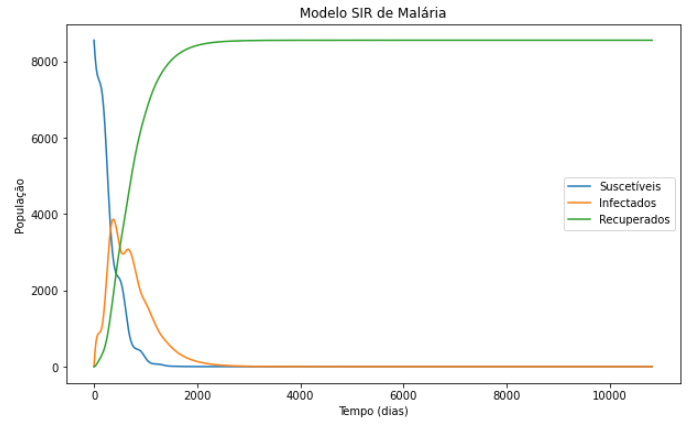
\includegraphics[scale=0.6] {SIR_R0_near1.png}}
        \caption{SIR com $T'=25.6 ^\circ C, \ A=15 \ (^\circ C^2 \ \text{dias})^{-1}, \ D_1=55 \ (^\circ C \ \text{dias}), \ b_2=0.2, \ \gamma=1/365$}
\end{figure} 
\begin{figure}[!ht]
        \centering
        \hbox{\hspace{3.5em} 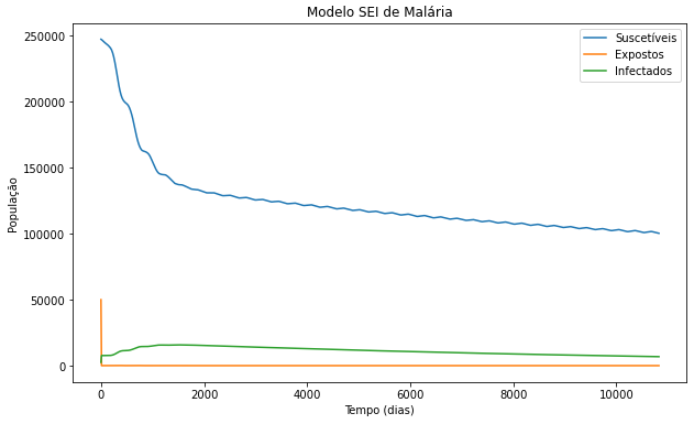
\includegraphics[scale=0.6] {SEI_R0_near1.png}}
        \caption{SEI com $T'=25.6 ^\circ C, \ A=15 \ (^\circ C^2 \ \text{dias})^{-1}, \ D_1=55 \ (^\circ C \ \text{dias}), \ b_2=0.2, \ \gamma=1/365$}
\end{figure}
\\\\
Discutindo essa aproximação de $\mathcal{R}_0$ a 1 com o orientador do 
Trabalho, foi decidido 
que ao invés de aumentar o valor $D_1$, um parâmetro empírico usado para 
estabilizar a taxa de picadas, seria ideal modificar $b_1$ e $b_2$, que são as
proporções de picadas gerando infecção em mosquitos e humanos suscetíveis, 
respectivamente, tendo em vista que, conforme temos mais ocorrências de áreas 
desmatadas, haverá um maior contato entre humanos e mosquitos, aumentando a 
proporção de picadas gerando infecção. 
\\\\
Junto com essa correção, também 
foram modelados os gráficos de evolução das taxas utilizadas, em função 
da temperatura e precipitação, ao invés do tempo, para que fosse 
possível analisar o comportamento dessas taxas conforme a temperatura e 
precipitação variam. Os gráficos estão indicados no apêndice, partindo do 15. 
Gerando esses gráficos, também foi percebido que seria ideal aumentar $R_L$ 
do valor atual de 312 mm para 450 mm, para evitar que a probabilidade de 
sobrevivência de mosquitos durante as diferentes fases se 
tornasse muito próximo de 0, o que estava afetando a taxa de 
nascimentos $b(R,T)$, e diminuir $\gamma$ de 1/365 dias para 1/120, valor original
do artigo de referência \cite{Parham2010}, de forma que a curva epidêmica fosse mais
próxima do analisado na realidade, visto na Figura 5 que a curva de infectados começa
a crescer logo no início da análise, e a infecção só deixa de ocorrer após mais de
5 anos.
\\\\
Após o desenvolvimento dos gráficos das taxas, foi iniciada a modelagem usando os dados 
``reais" da população obtidos através da interpolação dos dados de população de Manaus indicada na Tabela 4.
Com os valores previmente obtidos, a taxa anual de nascimentos foi estimada como sendo de 206.8 
nascimentos por ano. Sendo assim, são 0.56657 nascimentos por dia, aproximadamente, e 0.00007 nascimentos
diários por pessoa, já que a população rural média em Manaus é de aproximadamente 8078.5 pessoas entre 2004 e 2008.
\\\\
Assumindo que a taxa de natalidade e mortalidade de humanos é a mesma, foi então incluído na 
modelagem o parâmetro $\mu_H$, com valor 0.00007, representando a taxa diária de 
nascimentos e mortes. O modelo atualizado ficou como a seguir:
\begin{gather*}
\begin{cases}
\dfrac{dS_H}{dt} = \mu_HN-ab_2\bigg(\dfrac{I_M}{N}\bigg)S_H - \mu_HS_H\\
\\
\dfrac{dI_H}{dt} = ab_2\bigg(\dfrac{I_M}{N}\bigg)S_H-\gamma I_H - \mu_HI_H\\
\\
\dfrac{dR_H}{dt} = \gamma I_H - \mu_HR_H\\
\\
\end{cases}
\end{gather*}
A elaboração dos gráficos, a partir do Apêndice 27, foi feita em \footnote{https://github.com/RaphaLevy/TCC/blob/main/Modelagem\_com\_Dinamica\_Pop/ \\
Modelagem\_com\_Entrada\_Populacional.ipynb}.
\\\\
Tendo corrigido as equações, o $\mathcal{R}_0$ do SIR e do modelo acoplado 
foram $\Big | \dfrac{ab_2}{\gamma + \mu_H}\Big | $ e 
$\Big | \sqrt{\dfrac{a^2b_1b_2b_3}{(b_3+l+\mu)(\gamma+\mu_H)\mu}}\Big | $, respectivamente. Podemos verificar que $\mathcal{R}_0$ é de fato adimensional: $a, \ b_3, \ l, \ \mu$ e $\gamma$ são funções de unidade 1/dia, enquanto $b_1$ e $b_2$ são adimensionais. Sendo assim, $\mathcal{R}_0$ do SIR tem dimensão (1/dia)/(1/dia), $\mathcal{R}_0$ do SEI tem dimensão (1/dia$^2$)/(1/dia$^2$) e o acoplado tem dimensão (1/dia$^3$)/(1/dia$^3$). 
\\\
Como esperado, com $\mathcal{R}_0$ menor que 1, e apenas 1 mosquito exposto e 
1 humano infectado, a doença não consegue se estabelecer, como pode ser visto abaixo:
\begin{figure}[!ht]
        \centering
        \hbox{\hspace{2.5em} 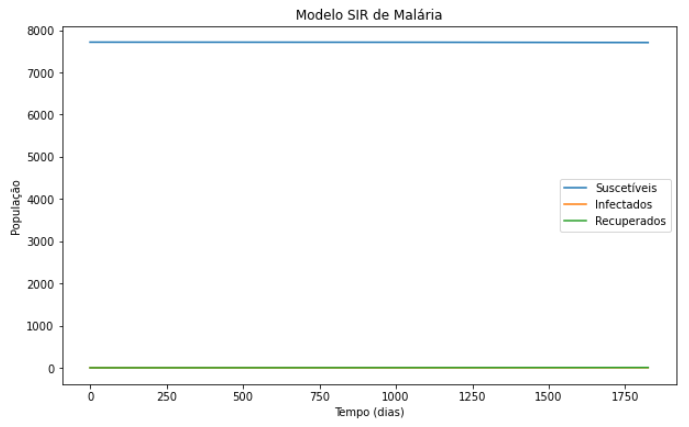
\includegraphics[scale=0.7] {SIR_Entrada_Pop_1_1_Infect.png}}
        \caption{SIR com $T'=25.6 ^\circ C, \ A=12.5 \ (^\circ C^2 \ \text{dias})^{-1}, \ B=15 \ (^\circ C \ \text{dias})^{-1}, \ C=-48.78 \ (\text{dias})^{-1}, \ R_L=450 \text{mm}, E_{M0}=1, I_{H0}=1$} 
\end{figure} 
\begin{figure}[!ht]
        \centering
        \hbox{\hspace{2.5em} 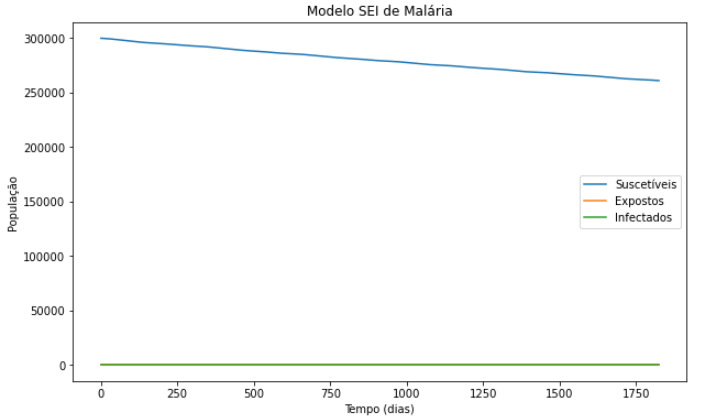
\includegraphics[scale=0.7] {SEI_Entrada_Pop_1_1_Infect.png}}
        \caption{SEI com $T'=25.6 ^\circ C, \ A=12.5 \ (^\circ C^2 \ \text{dias})^{-1}, \ B=15 \ (^\circ C \ \text{dias})^{-1}, \ C=-48.78 \ (\text{dias})^{-1}, \ R_L=450 \text{mm}, E_{M0}=1, I_{H0}=1$} 
\end{figure} 
\\Dos apêndices 27 a 30, aumentando o número de infectados e expostos, inicialmente com um 
``pequeno" aumento, com 1/30 da população de mosquitos exposta à doença, e 6.5\% 
de humanos infectados, a população de infectados humanos começa a aumentar, 
mas não consegue se estabelecer. Prolongando o tempo de análise, será possível 
ver que a população se extinguirá nos anos seguintes. Idealmente, seria 
possível verificar a população de infectados tendendo a 0 ainda no tempo da 
análise. Por outro lado, iniciando a população humana com cerca de 13\% de infectados, 
é possível ver que essa população tem um aumento ao longo do primeiro ano, 
chegando a quase 41\% da população, mas posteriormente decaindo.
\\\\
No caso dos mosquitos, a população inicial de expostos quase que 
imediatamente se torna de infectados, se estabilizando em cerca de 5000 
indivíduos, mas não é possível perceber a população de infectados se 
extinguindo, mesmo prolongando o tempo de análise. Esse comportamento 
ainda pode ser notado quando 1/3 da população começa exposto, rapidamente 
se tornando infectada, mas se estabelecendo em cerca de 10000 indivíduos. 
\\\\
Agora, voltando a um único exposto e infectado inicialmente, e incluindo um fator
multiplicativo $k$ nas proporções $b_1$ e $b_2$, representando o aumento de contato
entre humanos e mosquitos devido ao desmatamento, foi possível analisar o efeito desse impacto
na evolução da doença. A formulação final do modelo ficou como a seguir:
\begin{gather*}
\begin{cases}
\dfrac{dS_H}{dt} = \mu_HN-akb_2\bigg(\dfrac{I_M}{N}\bigg)S_H - \mu_HS_H\\
\\
\dfrac{dI_H}{dt} = akb_2\bigg(\dfrac{I_M}{N}\bigg)S_H-\gamma I_H - \mu_HI_H\\
\\
\dfrac{dR_H}{dt} = \gamma I_H - \mu_HR_H\\
\\
\dfrac{dS_M}{dt} = b - akb_1\bigg(\dfrac{I_H}{N}\bigg)S_M - \mu S_M\\
\\
\dfrac{dE_M}{dt} = akb_1\bigg(\dfrac{I_H}{N}\bigg)S_M - \mu E_M - b_3E_M -lE_M\\
\\
\dfrac{dI_M}{dt} = b_3E_M -\mu I_M\\
\end{cases}
\end{gather*}
Aumentando as proporções em 20 e 50\% ($k=1.2$ e $k=1.5$), não foi possível perceber
nenhuma diferença visível na evolução da doença, isso porque $\mathcal{R}_0 < 1$  
para $k < 2.0746963059512207$, como pode ser visto abaixo:
\begin{figure}[!ht]
        \centering
        \hbox{\hspace{3em} 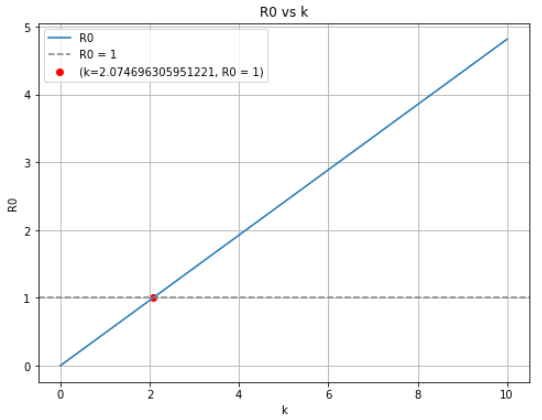
\includegraphics[scale=0.8] {Plot_R0_vs_k.png}}
        \caption{$\mathcal{R}_0$ em função de $k$}
\end{figure} 
\\\\
%mas com um aumento de 100\%, o resultado ficou como a seguir:
Sendo assim, mesmo um aumento de 100\% nas proporções de picadas causando infecção
não seria suficiente para que a doença se torne endêmica. Abaixo estão testes com $k=2.5, \ 5$ e $10$:
\begin{figure}[!ht]
        \centering
        \hbox{\hspace{2.0em} 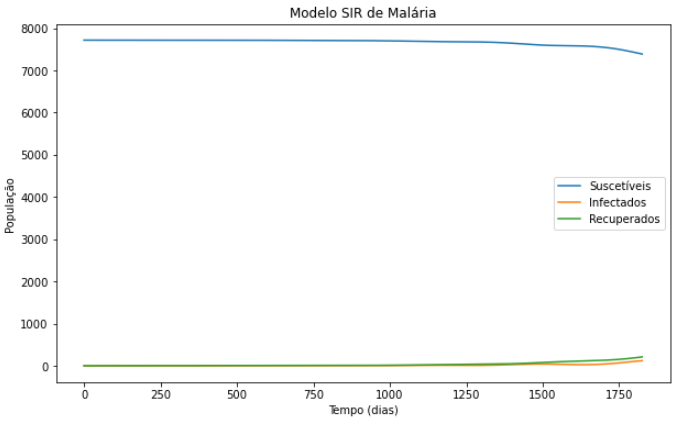
\includegraphics[scale=0.7] {Correcao_SIR_Desmat_k=2_5.png}}
        \caption{SIR com $T'=25.6 ^\circ C, \ A=12.5 \ (^\circ C^2 \ \text{dias})^{-1}, \ B=15 \ (^\circ C \ \text{dias})^{-1}, \ C=-48.78 \ (\text{dias})^{-1}, \ R_L=450 \text{mm}, \ k=2.5$}
\end{figure} 
\begin{figure}[!ht]
        \centering
        \hbox{\hspace{1.5em} 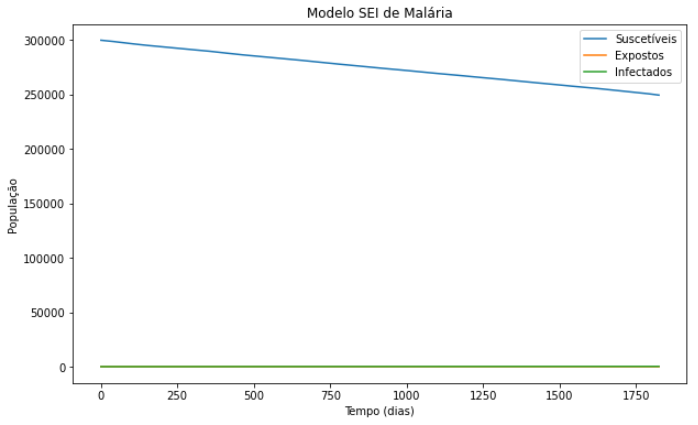
\includegraphics[scale=0.7] {Correcao_SEI_Desmat_k=2_5.png}}
        \caption{SEI com $T'=25.6 ^\circ C, \ A=12.5 \ (^\circ C^2 \ \text{dias})^{-1}, \ B=15 \ (^\circ C \ \text{dias})^{-1}, \ C=-48.78 \ (\text{dias})^{-1}, \ R_L=450 \text{mm}, \ k=2.5$}
\end{figure} 
\newpage
Aumentando em $150\%$ a proporção de picadas causando infecção, já é possível notar que o 
número de infectados começa a aumentar, ainda que quase no final do período 
de análise. Isso porque com o aumento em $k$, $\mathcal{R}_0$ passou de 0.48, 
com $k=1$, para 1.2, permitindo que a doença se estabeleça a longo prazo. Como $k$
está relacionado tanto com $b_1$ quanto $b_2$, esse fator aparecerá como $k^2$ no
numerador de $\mathcal{R}_0$, portanto afetando seu valor de forma linear.
Aumentando $k$ para 5, será bem mais perceptível a evolução da doença:
\begin{figure}[!ht]
        \centering
        \hbox{\hspace{3.7em} 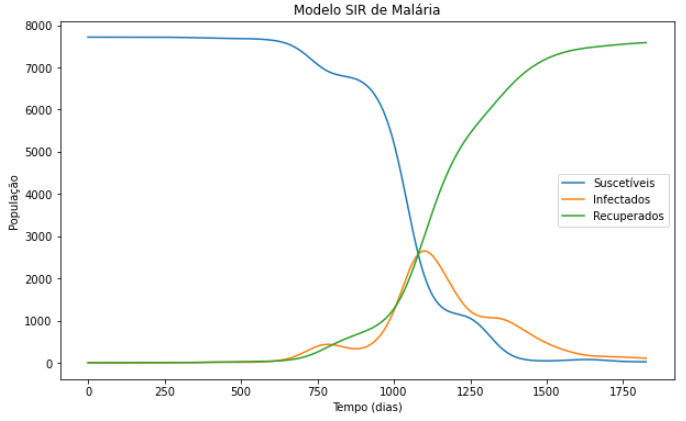
\includegraphics[scale=0.6] {Correcao_SIR_Desmat_k=5.png}}
        \caption{SIR com $T'=25.6 ^\circ C, \ A=12.5 \ (^\circ C^2 \ \text{dias})^{-1}, \ B=15 \ (^\circ C \ \text{dias})^{-1}, \ C=-48.78 \ (\text{dias})^{-1}, \ R_L=450 \text{mm}, \ k=5$}
\end{figure} 
\begin{figure}[!ht]
        \centering
        \hbox{\hspace{3.2em} 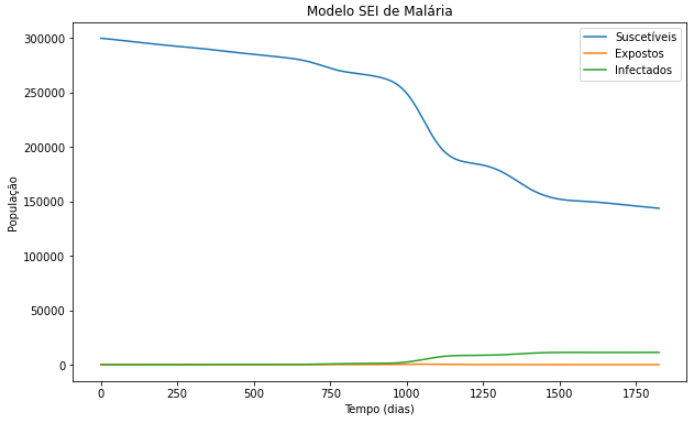
\includegraphics[scale=0.6] {Correcao_SEI_Desmat_k=5.png}}
        \caption{SEI com $T'=25.6 ^\circ C, \ A=12.5 \ (^\circ C^2 \ \text{dias})^{-1}, \ B=15 \ (^\circ C \ \text{dias})^{-1}, \ C=-48.78 \ (\text{dias})^{-1}, \ R_L=450 \text{mm}, \ k=5$}
\end{figure} 
\newpage
Nesse caso, $\mathcal{R}_0 = 2.41$, e apesar de não ser possível verificar no tempo 
máximo dos 5 anos, nesse caso o número de infectados consegue se estabilizar, 
oscilando em aproximadamente 50 humanos e 9000 mosquitos infectados. Aumentando $k$ para 10, 
$\mathcal{R}_0 = 4.82$, e a infecção atinge seu máximo de forma ainda mais rápida:
\begin{figure}[!ht]
        \centering
        \hbox{\hspace{4.2em} 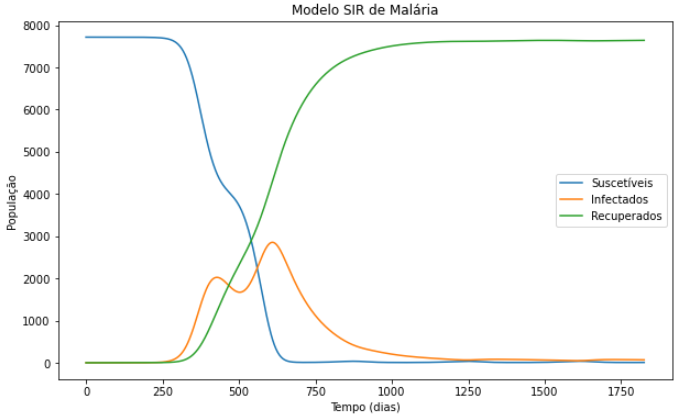
\includegraphics[scale=0.6] {Correcao_SIR_Desmat_k=10.png}}
        \caption{SIR com $T'=25.6 ^\circ C, \ A=12.5 \ (^\circ C^2 \ \text{dias})^{-1}, \ B=15 \ (^\circ C \ \text{dias})^{-1}, \ C=-48.78 \ (\text{dias})^{-1}, \ R_L=450 \text{mm}, \ k=10$}
\end{figure} 
\begin{figure}[!ht]
        \centering
        \hbox{\hspace{4.2em} 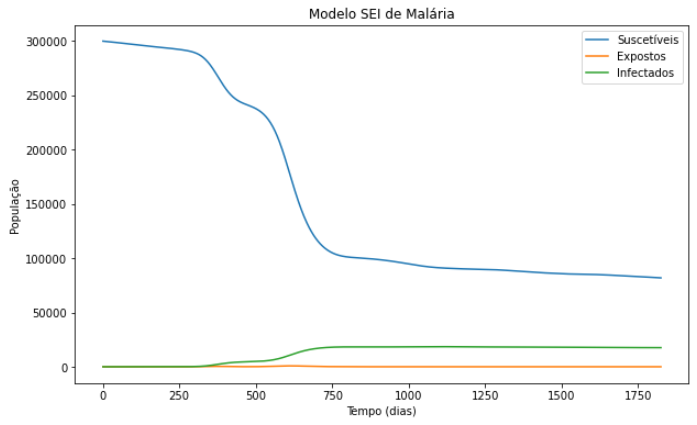
\includegraphics[scale=0.6] {Correcao_SEI_Desmat_k=10.png}}
        \caption{SEI com $T'=25.6 ^\circ C, \ A=12.5 \ (^\circ C^2 \ \text{dias})^{-1}, \ B=15 \ (^\circ C \ \text{dias})^{-1}, \ C=-48.78 \ (\text{dias})^{-1}, \ R_L=450 \text{mm}, \ k=10$}
\end{figure} 
\newpage
Com esses resultados, é possível perceber que o desmatamento acarretando em aproximação
entre hospedeiro e vetor causa um alto impacto na dinâmica da malária,
dado que mesmo com um único indivíduo infectado, a doença se estabelece e atinge 
um nível de infecção humana de cerca de $40\%$ da população conforme a 
proporção de picadas causando infecção aumenta. Agora, podemos encontrar qual é o valor de $I_H$
no equilíbrio dependendo de $k$:
\begin{figure}[!ht]
        \centering
        \hbox{\hspace{4.2em} 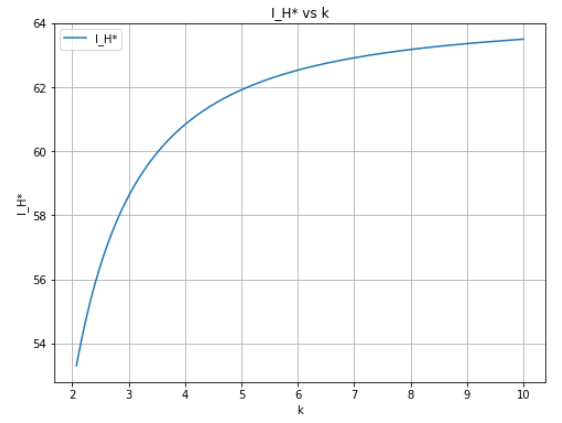
\includegraphics[scale=0.7] {Plot_I_H_vs_k.png}}
        \caption{$I_H^*$ em função de $k$}
\end{figure} 
\\\\
Iniciando o plot a partir de $k$ que deixa $\mathcal{R}_0 = 1$, é possível ver que
o equilíbrio endêmico da população humana se aproxima de 64 conforme $k$ se aproxima de 10.
Mais especificamente, quando $k=10$, $I_H^* \approx 63.49$ \footnote{A elaboração 
dos gráficos em função de $k$ podem ser encontrados em https://github.com/RaphaLevy/TCC/blob/main/Modelagem\_com\_Dinamica\_Pop/Plota\_Equilibrio\_e\_R0.ipynb. 
O cálculo dos equilíbrios pode ser encontrado em
https://github.com/RaphaLevy/TCC/blob/main/Modelagem\_com\_Dinamica\_Pop/R0\_com\_Dinamicas\_Demograficas.ipynb}.
Analisando o equilíbrio de suscetíveis conforme $k$ aumenta, é possível 
ver o equilíbrio decaindo rapidamente
de $N$ quando $k=0$ para aproximadamente 5000 indivíduos quando $k=1$. Analisando 
nos valores de $k$ tais que $\mathcal{R}_0 \geq 1$:
\begin{figure}[!ht]
        \centering
        \hbox{\hspace{4.2em} 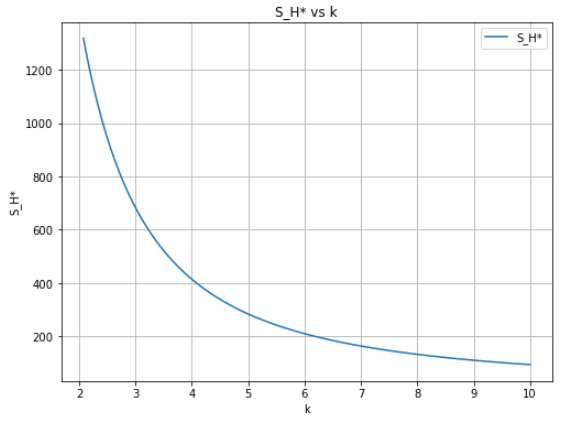
\includegraphics[scale=0.7] {Plot_S_H_vs_k.png}}
        \caption{$S_H^*$ em função de $k$}
\end{figure} 
\newpage
Nesse caso, a população de suscetíveis tende a aproximadamente 95 conforme 
$k$ se aproxima de 10. Tendo calculado os equilíbrios de $S_H$ e $I_H$,
foi possível fazer uma análise de estabilidade global. Como estamos interessados
em analisar o equilíbrio endêmico, utilizei $k=10$:
\begin{figure}[!ht]
        \centering
        \hbox{\hspace{2.2em} 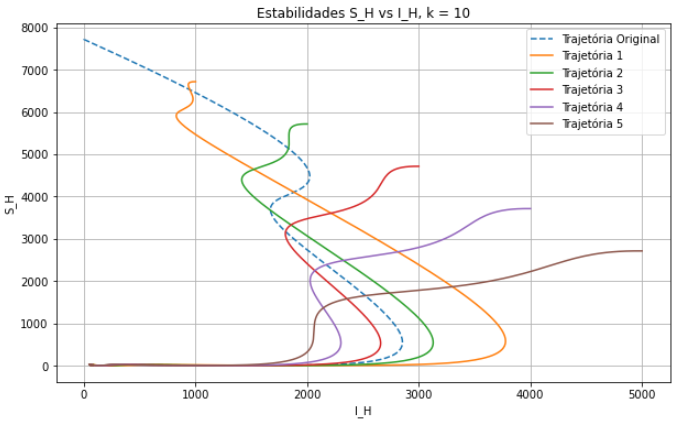
\includegraphics[scale=0.7] {Equilibrio_SH_IH_k_10.png}}
        \caption{Equilíbrio global $S_H^* \times I_H^*$ para $k=10$}
\end{figure}
\\\\
Nesse caso, foram feitas 6 análises, a primeira utilizando os
valores iniciais de $S_H$ e $I_H$ como sendo 7716 e 1, e as demais aumentando $I_H$ 
em 1000 e diminuindo $S_H$ em 1000 indivíduos. Nesse caso, é possível
ver as populações de suscetíveis e infectados com um equilíbrio final de
aproximadamente 8 e 70 pessoas, respectivamente. Com isso,
poderíamos comparar o resultado obtido com o cálculo do equilíbrio endêmico de Adda e Bichara
\cite{adda2011global}, onde
\begin{gather*}
        S_H^* = \dfrac{1}{\mathcal{R}_0} \\
        I_H^* = \dfrac{\mu_H}{\mu_H+\gamma}(1-\dfrac{1}{\mathcal{R}_0})
\end{gather*}       
Através desse cálculo, a população de suscetíveis e infectados no equilíbrio 
foi de aproximadamente 1601 e 51, respectivamente. Notavelmente, esses valores 
estão destoantes dos 
obtidos através do cálculo numérico. Contudo, é necessário considerar a principal diferença entre as equações
propostas para $S$ e $I$ nesse Trabalho e no artigo de Adda e Bichara, que é o uso de
$I_M$ na taxa de infecção $\beta$, dada a dinâmica do modelo 
acoplado de SIR e SEI nesse caso, que não está sendo considerada no trabalho
de Adda e Bichara.